\documentclass[12pt]{article}
\usepackage{tp}

\title{Préparation au concours ACM -- TP 2}
\author{Christoph Dürr \and Jill-Jênn Vie}
\date{September 25, 2014}

\begin{document}
\maketitle
\subsection*{Quelques conseils}

\begin{itemize}
\item Entraînez-vous à identifier les problèmes les plus faciles.
\item Lisez bien les contraintes d'affichage : faut-il un retour de ligne entre deux instances consécutives ou même à la fin ? Y a-t-il des deux-points, ou des points à la fin des phrases ?
\item Pensez aux cas extrêmes : que se passe-t-il lorsque le graphe est vide ? Lorsqu'il n'y a aucune instance ? Lorsque les entiers donnés en entrée sont négatifs ? Il peut être utile qu'un membre de votre équipe rédige des tests unitaires.
\item Aussi, pensez aux bornes sur les entiers : faut-il un \texttt{unsigned long long int} (\texttt{\%lld}) ?
\item Évaluez la complexité de votre idée d'algorithme avant de l'implémenter.
\item Attention à la mémoire : évitez d'utiliser \texttt{malloc} mais plutôt des instructions de type \texttt{vector<bool> dejaVu(nbNodes)}, ou n'hésitez pas à faire un tableau de taille suffisamment grande pour accueillir les instances lorsque les contraintes le permettent, quitte à ce que ce soit une variable globale.
\item S'il y a plusieurs instances, pensez à réinitialiser toutes les données à chaque nouvelle lecture, notamment si vous utilisez des variables globales.
\item Évitez d'utiliser des classes, éventuellement recodez vos propres structures si vous ne voulez pas utiliser \texttt{pair<int, int>} ou \texttt{tuple}. Un exemple d'implémentation minimale pour accueillir un graphe pondéré :
\begin{verbatim}
struct Node {
    int id;
    vector<pair<int, int> > neighbours;
};
vector<Node> graph(nb_nodes);
\end{verbatim}
\item Lorsque vous effectuez des comparaisons entre flottants, songez à conserver une tolérance de \texttt{1e-6}.
\end{itemize}

\problem{The 3n + 1 problem}


\noindent
UVA \no 100\bigskip

\subsection*{The Problem}

Problems in Computer Science are often classified as belonging to a
certain class of problems (e.g., NP, Unsolvable, Recursive).  In this
problem you will be analyzing a property of an algorithm whose
classification is not known for all possible inputs.

Consider the following algorithm:
\begin{enumerate}
    \item input n
    \item print n
    \item while $n\neq 1$:
    \begin{enumerate}
        \item if $n$ is odd, set $n:=3n+1$ else $n:=n/2$
        \item print n
    \end{enumerate}
\end{enumerate}

Given the input 22, the following sequence of numbers will be printed
22 11 34 17 52 26 13 40 20 10 5 16 8 4 2 1

It is conjectured that the algorithm above will terminate (when a 1 is
printed) for any integral
input value.  Despite the simplicity of the algorithm,
it is unknown whether this conjecture is true.  It has been verified,
however, for all integers $n$ such that $0\leq n\leq 1000000$  (and, in fact,
for many more numbers than this.)

Given an input $n$, it is possible to determine
the number of numbers printed (including
 the 1).  For a given $n$ this is
called the \emph{cycle-length} of $n$.  In the example above, the cycle
length of 22 is 16.

For any two numbers $i$ and $j$ you are to determine the maximum cycle
length over all numbers between $i$ and
$j$.



\subsection*{The Input}

The input will consist of a series of pairs of integers $i$ and $j$, one pair of
integers per line.  All integers will be less than 1,000,000 and greater
than 0.

You should process all pairs of integers and for each
pair determine the maximum cycle length over all integers between and
including $i$ and $j$.

You can assume that no operation overflows a 32-bit integer.


\subsection*{The Output}

For each pair of input integers $i$ and $j$ you should output $i$, $j$,
and the maximum cycle length for integers between and including
$i$ and $j$.  These three numbers
should be separated by at least one space with all three numbers on one
line and with one line of output for each line of input.  The integers
$i$ and $j$ must appear in the output in the same order in which they
appeared in the input and should be
followed by the maximum cycle length (on the same line).


\subsection*{Sample Input}
\begin{verbatim}
1 10
100 200
201 210
900 1000
\end{verbatim}

\subsection*{Sample Output}
\begin{verbatim}
1 10 20
100 200 125
201 210 89
900 1000 174
\end{verbatim}

\problem{Robot Motion}


\noindent
UVA \no 10116\bigskip

\subsection*{The Problem}

A robot has been programmed to follow the instructions in its path.
 Instructions for the next
direction the robot is to move are laid down in a grid.  The possible
instructions are

\begin{description}
    \item[N] north (up the page)
    \item[S] south (down the page)
    \item[E] east (to the right on the page)
    \item[W] west (to the left on the page)
\end{description}

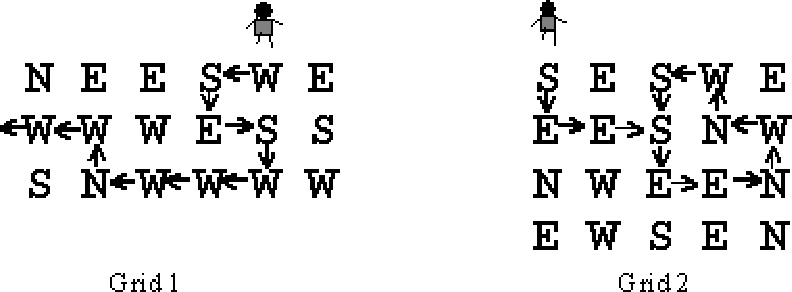
\includegraphics[width=12cm]{problems/p10116.pdf}

For example, suppose the robot starts on the north (top) side of Grid 1
and starts
south (down).  The path the robot follows is shown.  The robot goes through 
10 instructions
in the grid before leaving the grid.

Compare what happens in Grid 2:  the robot goes through 3  instructions
only once, and then
starts a loop through 8 instructions, and never exits.

You are to write a program that determines how long it takes a robot to get out of the grid or
how the robot loops around.



\subsection*{The Input}

There will be one or more grids for robots to navigate.  The data for
each is in the following form. On the first line are three integers
separated by blanks:  the number of rows in the grid, the number of
columns in the grid, and the number of the column in which the robot
enters from the north.  The possible entry columns are numbered starting
with one at the left.  Then come the rows of the direction instructions.
Each grid will have at least one and at most 10 rows and columns
of instructions.  The lines of instructions contain only the characters
N,S,E or W
with no blanks.

The end of  input is indicated by a row containing 0 0 0.
 
\subsection*{The Output}

For each grid in the input there is one line of output.  Either the robot
follows a certain
number of  instructions and exits the grid on any one the four sides or
else the robot follows
the instructions on a certain number of locations once, and then the
instructions on some
number of locations repeatedly. The sample input below corresponds to the
two grids above
and illustrates the two forms of output.  
The word "step" is
always
immediately followed by "(s)" whether or not the number before it is 1.

\subsection*{Sample Input}
\begin{verbatim}
3 6 5
NEESWE
WWWESS
SNWWWW
4 5 1
SESWE
EESNW
NWEEN
EWSEN
0 0 0    
\end{verbatim}

\subsection*{Sample Output}
\begin{verbatim}
10 step(s) to exit
3 step(s) before a loop of 8 step(s) 
\end{verbatim}


\problem{Anagram}


\noindent
UVA \no 195\bigskip

\subsection*{The Problem}

You are to write a program that has to generate all possible words from
a given set of letters.

\paragraph{Example:}
Given the word "abc", your program should - by exploring all different
combination of the three letters - output the words "abc", "acb",
"bac", "bca", "cab" and "cba".

In the word taken from the input file, some letters may appear more than
once. For a given word, your program should not produce the same word more
than once, and the words should be output in alphabetically ascending order.



\subsection*{The Input}

The input file consists of several words. The first line contains a number
giving the number of words to follow. Each following line contains one word.
A word consists of uppercase or lowercase letters from A to Z. Uppercase
and lowercase letters are to be considered different.

\subsection*{The Output}

For each word in the input file, the output file should contain all different
words that can be generated with the letters of the given word. The words
generated from the same input word should be output in alphabetically ascending
order. An upper case letter goes before the corresponding lower case letter.


\subsection*{Sample Input}
\begin{verbatim}
aAb
abc
acba
\end{verbatim}

\subsection*{Sample Output}
\begin{verbatim}
Aab
Aba
aAb
abA
bAa
baA
abc
acb
bac
bca
cab
cba
aabc
aacb
abac
abca
acab
acba
baac
baca
bcaa
caab
caba
cbaa
\end{verbatim}
\problem{Ordering Tasks}

\noindent
UVa 10305\bigskip

John has $n$ tasks to do.
Unfortunately, the tasks are not independent and the execution of one task is only
possible if other tasks have already been executed. 


\subsection*{The Input}

The input will consist of several instances of
the problem. Each instance begins with a line containing two integers, $1\leq n\leq 100$ and $m$. $n$
is the number of tasks (numbered from 1
to $n$) and $m$ is the number of direct precedence relations between tasks. After
this, there will be $m$ lines with two
integers $i$ and $j$, representing the fact that task $i$ must be executed before task $j$.
An instance with $n = m = 0$ will
finish the input. 


\subsection*{The Output}

For each instance,
print a line with $n$ integers representing the tasks in a possible order of execution.



\subsection*{Sample Input}
\begin{verbatim}
5 4
1 2
2 3
1 3
1 5
0 0
\end{verbatim}

\subsection*{Sample Output}
\begin{verbatim}
1 4 2 5 3
\end{verbatim}

% http://uva.onlinejudge.org/index.php?option=com_onlinejudge&Itemid=8&page=show_problem&problem=3989

\problem{Beehives}

\noindent
UVa 12544 (SWERC 2012)\bigskip

Bees are one of the most industrious insects. Since they collect nectar and pollen from flowers, they have to rely on the trees in the forest. For simplicity they numbered the $n$ trees from $0$ to $n - 1$. Instead of roaming around all over the forest, they use a particular list of paths. A path is based on two trees, and they can move either way i.e. from one tree to another in straight line. They don't use paths that are not in their list.

As technology has been improved a lot, they also changed their working strategy. Instead of hovering over all the trees in the forest, they are targeting particular trees, mainly trees with lots of flowers. So, they planned that they will build some new hives in some targeted trees. After that they will only collect their foods from these trees. They will also remove some paths from their list so that they don't have to go to a tree with no hive in it.

Now, they want to build the hives such that if one of the paths in their new list go down (some birds or animals disturbs them in that path) it's still possible to go from any hive to another using the existing paths.

They don't want to choose less than two trees and as hive-building requires a lot of work, they need to keep the number of hives as low as possible. Now you are given the trees with the paths they use, your task is to propose a new bee hive colony for them.

\subsection*{Input}

Input starts with an integer $T$ ($T \leqslant 50$), denoting the number of test cases.

Each case starts with a blank line. Next line contains two integers $n$ ($2 \leqslant n \leqslant 500$) and $m$
($0 \leqslant m \leqslant 20000$), where $n$ denotes the number of trees and $m$ denotes the number of paths. Each of the next $m$ lines contains two integers $u$ $v$ ($0 \leqslant u$, $v < n$, $u \neq v$) meaning that there is a path between tree $u$ and $v$. Assume that there can be at most one path between tree $u$ to $v$, and needless to say that a path will not be given more than once in the input.

\subsection*{Output}

For each case, print the case number and the number of beehives in the proposed colony or `impossible' if its impossible to find such a colony.\bigskip

\textbf{NOTE:} Dataset is huge. Use faster I/O methods.
\bigskip

\begin{multicols}{3}
\subsection*{Sample Input 1}

\begin{verbatim}
3

3 3
0 1
1 2
2 0

2 1
0 1
\end{verbatim}
\columnbreak
~\vspace{1cm}

\begin{verbatim}
5 6
0 1
1 2
1 3
2 3
0 4
3 4
\end{verbatim}
\columnbreak
\subsection*{Sample Output}

\begin{verbatim}
Case 1: 3
Case 2: impossible
Case 3: 3
\end{verbatim}
\end{multicols}

\end{document}
